\begin{table*}[!t]
  \caption{Regime~A (N-BaIoT, $K=9$): primary controlled results.}
  \label{tab:regime_a}
  \centering
  \begingroup
  \footnotesize
  \setlength{\tabcolsep}{3pt}%
  \renewcommand{\arraystretch}{1.15}%
  \begin{tabular*}{\textwidth}{@{\extracolsep{\fill}}l c c c c c c c}
    \toprule
    Baseline & Mean FPR & Mean TPR & CV(FPR) & CV(TPR) & Worst~BA & Mean~F1 & P10~F1 \\
    \midrule
    B0 (Centralized)    & $0.057\pm0.001$ & $0.829\pm0.037$ & $0.787\pm0.031$ & $0.278\pm0.036$ & $0.653\pm0.010$ & $0.720\pm0.054$ & $0.403\pm0.059$ \\
    B1 (Client-Averaged) & $0.039\pm0.002$ & $0.738\pm0.050$ & $\mathbf{1.017\pm0.019}$ & $0.289\pm0.029$ & $0.649\pm0.011$ & $0.563\pm0.068$ & $0.344\pm0.062$ \\
    B2 (Per-Client)     & $0.043\pm0.001$ & $0.744\pm0.019$ & $\mathbf{0.299\pm0.073}$ & $0.336\pm0.007$ & $0.651\pm0.001$ & $0.604\pm0.042$ & $0.300\pm0.000$ \\
    B3 (Family-Mean)    & $0.051\pm0.006$ & $0.745\pm0.018$ & $0.964\pm0.096$ & $0.336\pm0.007$ & $0.653\pm0.004$ & $0.606\pm0.038$ & $0.299\pm0.000$ \\
    B4 (Cluster-Mean)   & $0.044\pm0.003$ & $0.718\pm0.019$ & $0.645\pm0.045$ & $0.322\pm0.012$ & $0.654\pm0.007$ & $0.545\pm0.036$ & $0.299\pm0.000$ \\
    \bottomrule
  \end{tabular*}
  \par\vspace{4pt}
  \parbox{\textwidth}{\footnotesize Coverage 9/9, pending 0. Values are mean $\pm$ std over 5 seeds. B0 is a centralized reference and is excluded from the B1--B4 controlled ladder. Worst BA = worst-client balanced accuracy; Mean F1 = mean Macro-F1; P10 F1 = 10th-percentile Macro-F1 across eligible clients.}
  \par\vspace{2pt}
  \parbox{\textwidth}{\footnotesize Primary result: \textbf{B1$-$B2 CV(FPR) $\boldsymbol{\Delta = +0.718}$}, SD$\,{=}\,0.079$, seed range $[0.588,\,0.772]$, all 5 deltas positive; B1$-$B4 $\Delta = +0.372$, SD$\,{=}\,0.055$, seed range $[0.319,\,0.443]$.}
  \endgroup
\end{table*}

\section{Results and Discussion}
\label{sec:results}

\subsection{RQ1: FPR Dispersion Under the Client-Averaged Shared Threshold}

Table~\ref{tab:regime_a} presents aggregate results for Regime~A over 5 seeds.
Under B1, CV(FPR) is $1.017 \pm 0.019$---per-client FPRs vary by more than their mean
(a CV above 1 indicates high relative dispersion).
The natural N-BaIoT B1 CV(FPR) ($1.017$) substantially exceeds the IID Dirichlet
baseline ($0.074$), a difference of $0.943$, consistent with device heterogeneity
contributing to the observed dispersion.
B0's CV(FPR) ($0.787$), although lower than B1's, remains substantially above B2 ($0.299$),
consistent with any single pooled or shared scalar threshold crossing heterogeneous
device-error distributions at different exceedance fractions; B0 is included only as a
centralized privacy-incompatible reference, not as part of the controlled B1--B4 ladder.

Fig.~\ref{fig:regime-a-client-fpr} shows per-client FPR distributions.
The worst client (SimpleHome XCS7 security camera) reaches a mean FPR of approximately
$0.122$ while other clients operate near zero, illustrating the unequal alarm-rate
burden imposed by a single shared threshold across heterogeneous devices.

\subsection{RQ2: Held-Out FPR-Dispersion Reduction and Detection-Quality Cost}

The primary endpoint is the B1 vs.\ B2 CV(FPR) delta per seed.
Across the five planned seeds, the B1--B2 CV(FPR) deltas are all positive,
with mean $\Delta = 0.718$, SD$\,{=}\,0.079$, and range $[0.588,\, 0.772]$
(Table~\ref{tab:per_seed}).
These seed summaries are reported descriptively rather than as confidence intervals.
A supplementary bootstrap CI (10{,}000 resamples of the five seed-level deltas)
yields $[0.647,\, 0.769]$ at 95\%, excluding zero; given five seeds this is
treated as seed-level consistency evidence under the tested protocol.

Per-client calibration (B2) reduces CV(FPR) from $1.017$ to $0.299$ (coverage: 9/9, pending: 0).
B2 reduces CV(FPR) by 0.718 absolute units, corresponding to a relative reduction
$(\mathrm{CV}_{B1}-\mathrm{CV}_{B2})/\mathrm{CV}_{B1}=70.6\%$,
achieved with zero additional threshold uplink.
Operationally, B2 requires local threshold storage, versioning with the encoder/calibration window, and sufficient benign calibration data;
B4 requires transmitting the 4-scalar fingerprint per client.

The tradeoff with detection uniformity is clear from Table~\ref{tab:regime_a}:
CV(TPR) rises under B2 ($0.336$ vs.\ B1's $0.289$),
worst-client balanced accuracy is comparable (B1: $0.649$, B2: $0.651$),
and mean Macro-F1 improves ($0.604$ vs.\ $0.563$).
However, $P_{10}$ Macro-F1 falls from $0.344$ (B1) to $0.300$ (B2).
B2 slightly increases mean FPR ($0.043$ vs.\ $0.039$) but redistributes
false alarms more evenly; B1 attains a lower fleet-average FPR partly by concentrating
false alarms on high-variance clients.
The near-identical P10 Macro-F1 across B2--B4 ($\approx 0.300$, std $< 0.001$)
reflects a floor effect: the Ennio Doorbell client determines the P10 floor
under B2--B4 in all seeds.
Table~\ref{tab:failure_modes} provides the compact client-level separation diagnostic for the two limiting cases: Ennio Doorbell explains the lower-tail Macro-F1 loss under B2, while SimpleHome XCS7 explains the high-FPR tail under B1.

\begin{table}[t]
  \caption{Client-specific separation diagnostics explaining the main lower-tail Macro-F1 and FPR effects (Regime~A, 5-seed averages).}
  \label{tab:failure_modes}
  \centering
  \footnotesize
  \renewcommand{\arraystretch}{1.3}%
  \setlength{\tabcolsep}{4pt}%
  \begin{tabular}{@{}>{\raggedright\arraybackslash}p{1.8cm}>{\raggedright\arraybackslash}p{1.7cm}>{\raggedright\arraybackslash}p{2.0cm}>{\raggedright\arraybackslash}p{2.2cm}@{}}
    \toprule
    Client & Issue & Evidence & Interpretation \\
    \midrule
    SimpleHome XCS7 & Highest FPR under~B1 & Mean FPR ${\approx}\,0.122$ (worst client) & Shared~$\tau$ concentrates false alarms on high-variance devices \\[3pt]
    Ennio Doorbell & P10 Macro-F1 floor under B2--B4 & Lowest AUROC (0.931); 64.9\% attack mass below~$p_{95}$ & Benign/attack overlap limits detection after personalization \\
    \bottomrule
  \end{tabular}
\end{table}

Local thresholding controls Ennio's benign false alarms at the cost of
missing the majority of its low-magnitude attack traffic, explaining the P10 Macro-F1
floor.

\textbf{Mechanism.}
Per-client $p_{95}$ thresholding aligns each client's benign tail, mechanically
equalizing false-alarm rates on benign test traffic.
However, attack reconstruction-error distributions need not shift in parallel
with benign distributions: raising the threshold reduces benign false alarms
but can swallow low-magnitude anomaly scores, reducing TPR or lower-tail
Macro-F1 (Fig.~\ref{fig:mechanism} illustrates the benign-side mechanism).
B2 should therefore be interpreted as an FPR-dispersion calibration policy,
not a uniform detection-quality improvement.

All five seed-level deltas are positive (range $0.588$--$0.772$, Table~\ref{tab:per_seed}).

\begin{table}[t]
  \caption{Per-seed CV(FPR) and deltas, Regime~A.
           All $\Delta_{\text{B1-B2}}$ values are positive.
           B4 recovery $= (\text{B1} - \text{B4}) / (\text{B1} - \text{B2})$.
           Rows are paired by seed, so each B1--B2 delta compares threshold policies on the same frozen AE and score artifacts.}
  \label{tab:per_seed}
  \centering
  \footnotesize
  \renewcommand{\arraystretch}{1.2}%
  \setlength{\tabcolsep}{4pt}%
  \begin{tabular}{cccccc}
    \toprule
    Seed & B1 & B2 & B4 & $\Delta_{\text{B1-B2}}$ & B4 Recov.\ (\%) \\
    \midrule
    0 & 1.045 & 0.347 & 0.632 & $+0.698$ & 59.2 \\
    1 & 1.017 & 0.251 & 0.693 & $+0.765$ & 42.3 \\
    2 & 1.015 & 0.243 & 0.654 & $+0.772$ & 46.6 \\
    3 & 1.018 & 0.251 & 0.575 & $+0.767$ & 57.8 \\
    4 & 0.992 & 0.404 & 0.673 & $+0.588$ & 54.3 \\
    \midrule
    Mean & 1.017 & 0.299 & 0.645 & $+0.718$ & 51.8 \\
    \bottomrule
  \end{tabular}
\end{table}

Absolute FPR dispersion shows the same B1$>$B2 ordering:
IQR(FPR) decreases from $0.035\pm0.002$ (B1) to $0.015\pm0.003$ (B2),
and the max--min FPR gap narrows from $0.120\pm0.007$ to $0.041\pm0.012$.
Because CV(FPR) can be sensitive when mean FPR is small (mean FPR under B1: $0.039$;
under B2: $0.043$), absolute dispersion measures are reported alongside it throughout.
For B1, CV(FPR)$\,{=}\,1.017$ and mean FPR$\,{=}\,0.039$ imply $\sigma_{\text{FPR}} \approx 0.040$;
the CV above~1 therefore reflects genuine cross-client spread comparable to the mean,
not only a small-denominator artifact.

\textbf{Shared-threshold construction sensitivity.}
Pooled and sample-weighted shared-threshold variants preserve the B2 advantage
(Table~\ref{tab:sensitivity_shared}), suggesting the B1-to-B2 reduction is not
driven solely by the arithmetic-mean construction.

\begin{table}[t]
  \caption{Regime~A: shared-threshold construction sensitivity.}
  \label{tab:sensitivity_shared}
  \centering
  \footnotesize
  \setlength{\tabcolsep}{3pt}%
  \renewcommand{\arraystretch}{1.15}%
  \begin{tabular}{@{}llccc c@{}}
    \toprule
    Rule & Construction & CV(FPR) & IQR & \makecell{Max--min\\FPR} & $\Delta$ \\
    \midrule
    B1 & Arith.\ mean & $1.017{\pm.019}$ & $.035{\pm.002}$ & $.120{\pm.007}$ & $+.718$ \\
    B1-pool & Pooled $p_{95}$ & $0.805{\pm.048}$ & $.084{\pm.007}$ & $.134{\pm.012}$ & $+.506$ \\
    B1-wt & Wt.\ mean & $0.907{\pm.033}$ & $.050{\pm.018}$ & $.129{\pm.003}$ & $+.608$ \\
    B2 & Per-client $p_{95}$ & $0.299{\pm.073}$ & $.015{\pm.003}$ & $.041{\pm.012}$ & --- \\
    \bottomrule
  \end{tabular}
  \par\vspace{3pt}
  \parbox{\columnwidth}{\footnotesize Values: mean $\pm$ std, 5 seeds ($q=0.95$). No AE retraining; B1-pool = pooled $p_{95}$; B1-wt = sample-weighted mean of local $p_{95}$. $\Delta$ = vs B2. All B1 variants show larger CV(FPR) than B2, consistent with the advantage not being driven solely by arithmetic-mean construction. B1-pooled has lower CV but higher IQR: raising mean FPR reduces relative dispersion while absolute spread remains larger.}
\end{table}

\begin{figure}[t]
  \centering
  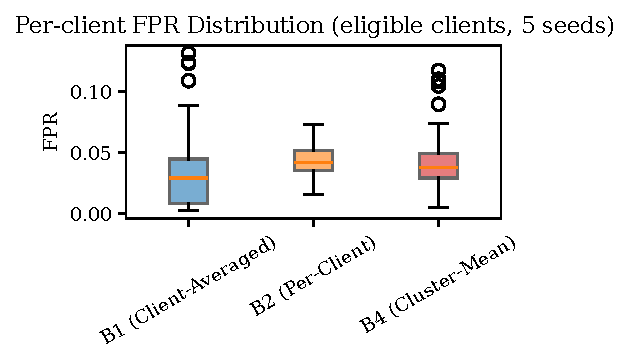
\includegraphics[width=\columnwidth]{figures/figure_3.pdf}
  \caption{Per-client FPR distributions under B1, B2, and B4 (Regime~A, pooled over 5 seeds).
           Descriptive only; inference uses seed-level deltas reported in text.}
  \label{fig:regime-a-client-fpr}
\end{figure}

\subsection{RQ3: Partial Recovery by Cluster-Mean Calibration}

Cluster-mean calibration (B4) achieves CV(FPR) $= 0.645 \pm 0.045$, a partial but consistent improvement over B1.
All five B1$-$B4 deltas are positive (mean $\Delta=0.372$, SD$\,{=}\,0.055$, range $[0.319,\,0.443]$);
all five B4$-$B2 deltas are also positive (mean $\Delta=0.346$, range $[0.269,\,0.442]$).
B4 recovers approximately $52\%$ of B2's improvement (per-seed: $42\%$--$59\%$, Table~\ref{tab:per_seed}).
B4 requires no device taxonomy and transmits only compact 4-scalar fingerprints per client;
however, it does not provide privacy (see Section~\ref{sec:framework}).
Cluster assignments show moderate stability across seeds in Regime~A
(pairwise adjusted Rand index: mean~$0.79$, range $[0.64,\,1.0]$ over all seed pairs).
A post-hoc silhouette check over $K \in \{2,3,4,5\}$ yields mean scores of
$0.29$, $0.31$, $0.34$, and $0.32$ respectively---all low and within $\pm 0.05$---confirming
that the nine-device Regime~A fingerprint space has no clearly dominant cluster count;
$K{=}3$ is a pragmatic fixed choice rather than a structurally optimal partition.
With only nine physical devices, B4 is exploratory and requires validation on larger fleets.
B4's fingerprint still depends on calibration-error statistics including $p_{95}$, so
clients below the eligibility threshold remain calibration-pending and use
$\tau_{\text{global}}$.

Family-mean calibration (B3, Regime~A only) reduces CV(FPR) negligibly
($0.964$ vs.\ B1's $1.017$): the coarse N-BaIoT device-family taxonomy
(Danmini/Ennio doorbells, Ecobee thermostat, Philips baby monitor, Samsung webcam,
Provision/SimpleHome security cameras) does not align with the reconstruction-error
calibration structure---devices within the same family can have dissimilar
benign-error distributions, while devices across families can be similar.
This taxonomy-independence of calibration structure motivates B4's data-driven clustering
over B3's label-based grouping.

\subsection{Regime B: File-Level Applicability Check (CICIoT2023)}

Table~\ref{tab:regime_b} shows Regime~B results.
Under the file-level CICIoT2023 partition, benign reconstruction-error distributions are
near-homogeneous (pairwise JS divergence: mean $0.004$, median $0.003$, max $0.038$
over all $\binom{63}{2}$ pairs and 5 seeds); these low pairwise JS values provide the compact calibration-distribution evidence for the Regime~B near-homogeneity interpretation.
B1 achieves CV(FPR) $= 0.099 \pm 0.002$; B2 increases it to $0.133 \pm 0.007$
(all five seed-level B1$-$B2 deltas are negative; mean $-0.034$, SD $0.006$, range $[-0.043,\,-0.026]$).
When benign distributions are near-homogeneous under this file-level partition, the shared
threshold is already a good fit and per-client calibration introduces variance without
benefit---no personalization improvement was observed in this setting.

\textbf{Interpretation caveat.}
Regime~B uses file-defined CICIoT2023 pseudo-clients (not physical devices) with randomized ordering; it is interpreted only as a near-homogeneous applicability boundary.
Intermediate-round score files are not reported; therefore, Regime~B is interpreted as a controlled threshold-scope check under a shared final frozen AE, with Macro-F1 stable at approximately 0.959 across threshold strategies, not as a convergence-quality claim.

\begin{table*}[t]
  \caption{Regime~B (\CICIoT{} file-defined clients, $K=63$, coverage~63/63, pending~0): mean $\pm$ std over
           5 seeds, eligible clients only. B3 not applicable. All runs budget-capped at 150 rounds.}
  \label{tab:regime_b}
  \centering
  \footnotesize
  \setlength{\tabcolsep}{5pt}%
  \renewcommand{\arraystretch}{1.2}%
  \begin{tabular*}{\textwidth}{@{\extracolsep{\fill}}l c c c c c c}
    \toprule
    Baseline & Mean FPR & Mean TPR & CV(FPR) & CV(TPR) & Worst~BA & Mean~F1 \\
    \midrule
    B0 (Centralized)     & $0.051\pm0.001$ & $0.981\pm0.000$ & $0.109\pm0.020$ & $0.001\pm0.000$ & $0.954\pm0.006$ & $0.959\pm0.000$ \\
    B1 (Client-Averaged) & $0.051\pm0.001$ & $0.982\pm0.000$ & $\mathbf{0.099\pm0.002}$ & $0.001\pm0.000$ & $0.959\pm0.002$ & $0.959\pm0.000$ \\
    B2 (Per-Client)      & $0.051\pm0.001$ & $0.982\pm0.000$ & $0.133\pm0.007$ & $0.001\pm0.000$ & $0.956\pm0.001$ & $0.959\pm0.000$ \\
    B4 (Cluster-Mean)    & $0.051\pm0.001$ & $0.982\pm0.000$ & $0.101\pm0.003$ & $0.001\pm0.000$ & $0.959\pm0.002$ & $0.959\pm0.000$ \\
    \bottomrule
  \end{tabular*}
  \par\vspace{3pt}
  \parbox{\textwidth}{\footnotesize Near-homogeneous regime: pairwise JS divergence mean $0.004$, max $0.038$. B1 achieves lowest CV(FPR); per-client calibration introduces variance without benefit under this partition.}
\end{table*}

\subsection{Regime C: Non-IID Severity Sweep}

Fig.~\ref{fig:severity} and Table~\ref{tab:regime_c} show that the personalization benefit is broadly consistent with larger gains under stronger
heterogeneity, concentrated in the low-$\alpha$ band and absent under near-IID conditions.
Table~\ref{tab:regime_c} reports the corresponding seed ranges, so Fig.~\ref{fig:severity} should be read descriptively rather than as a paired-seed trajectory.
The $\alpha=0.1$ and $\alpha=0.3$ seed ranges overlap ($[0.535,\,0.786]$ vs.\ $[0.420,\,0.897]$),
so strict monotonicity between these two levels should not be inferred from this data;
they form a high-heterogeneity band rather than a strictly ordered pair.
B4 follows the same qualitative pattern but remains a partial approximation.

\begin{figure}[t]
  \centering
  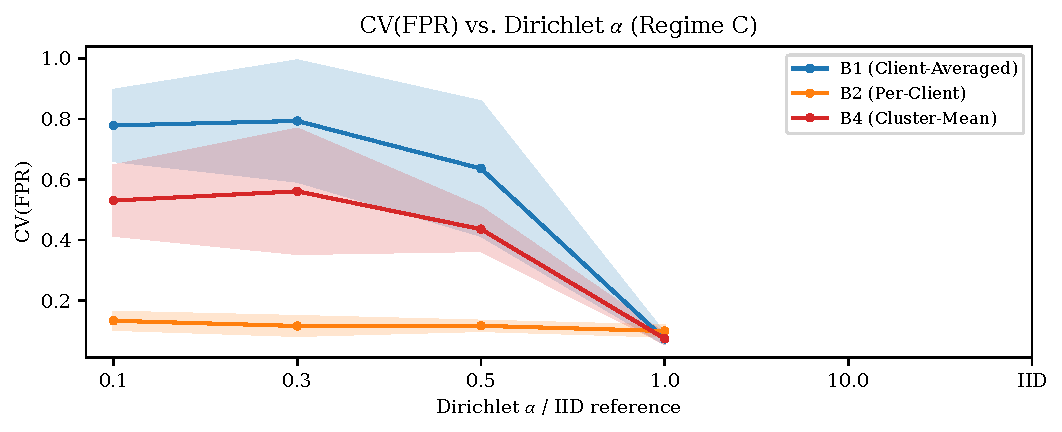
\includegraphics[width=\columnwidth]{figures/figure_4.pdf}
  \caption{Regime C: mean CV(FPR) by threshold strategy as a function of Dirichlet~$\alpha$.
           Whiskers show $\pm$1 std over 5 seeds.
           The B1--B2 gap is largest in the low-$\alpha$ band
           and disappears under IID or near-homogeneous conditions.}
  \label{fig:severity}
\end{figure}

\begin{table}[t]
  \caption{Regime C (N-BaIoT Dirichlet, $K=20$): CV(FPR) sweep.}
  \label{tab:regime_c}
  \centering
  \footnotesize
  \setlength{\tabcolsep}{0.75pt}%
  \renewcommand{\arraystretch}{1.15}%
  \begin{tabular}{@{}l c c c c l@{}}
    \toprule
    $\alpha$ & B1 CV & B2 CV & B4 CV & $\Delta$ & Seed range \\
    \midrule
    0.1  & $.779\pm.104$ & $.134\pm.025$ & $.531\pm.103$ & $0.645$ & $[0.535,\,0.786]$ \\
    0.3  & $.793\pm.178$ & $.117\pm.028$ & $.561\pm.184$ & $0.677$ & $[0.420,\,0.897]$ \\
    0.5  & $.636\pm.197$ & $.117\pm.014$ & $.436\pm.063$ & $0.519$ & $[0.240,\,0.777]$ \\
    1.0  & $.544\pm.116$ & $.096\pm.021$ & $.426\pm.066$ & $0.448$ & $[0.238,\,0.565]$ \\
    10.0 & $.174\pm.053$ & $.111\pm.016$ & $.133\pm.012$ & $0.063$ & $[0.006,\,0.122]$ \\
    IID  & $.074\pm.014$ & $.100\pm.015$ & $.075\pm.013$ & $-0.026$ & $[-0.032,\,-0.019]$ \\
    \bottomrule
  \end{tabular}
  \par\vspace{3pt}
  \parbox{\columnwidth}{\footnotesize Values are mean CV(FPR) $\pm$ std over 5 seeds. Mean FPR $\approx 0.050$ for all levels and baselines. B0 excluded. Coverage 20/20 (pending 0) except $\alpha{=}0.1$ (19--20/20, pending 0--1). $\Delta$\,=\,B1$-$B2 mean delta. Seed range = descriptive min--max over five seeds, not a confidence interval.}
\end{table}
